% Basic security concepts
\chapter{Network Security Concepts}
In this chapter we will go over the basic concepts of network and security, such as various kinds
of networks and the possible attacks that can be performed on them.
\begin{section}{Wireless Networks}
  A wireless communication network is a \textbf{computer network} that uses wireless data connections
  between network nodes. This means that most of the links are wireless.\\
  Some of the most common wireless networks are:
  \begin{itemize}
    \item Cellular networks
    \item Wireless local area networks (WLAN), such as Wi-Fi ones
    \item Wireless ad-hoc networks, such as bluetooth
    \item Vehicular networks
    \item Sensor networks
    \item Satellite networks
  \end{itemize}
  Historically the whole network infrastructure was wired, having limited mobility and flexibility.
  User equipment used to be directly connected to a network switch or a router through physical cables,
  and this is still true for many networks, for example in a data center and the core of the network.\\
  Nowadays, the situation is different, in fact the only wired component is the core of the network,
  while the edge of the communication infrastructure deploys wireless components.
  \begin{figure}[H]
    \centering
    \subfloat[Traditional wired network]{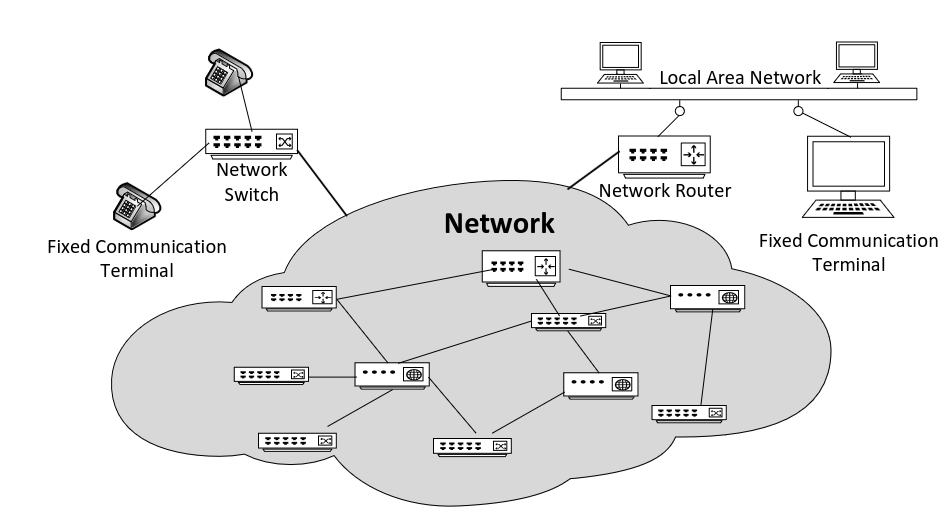
\includegraphics[width=0.5\textwidth]{img/wireless/wired network.png}}
    \hfill
    \subfloat[Modern wireless network]{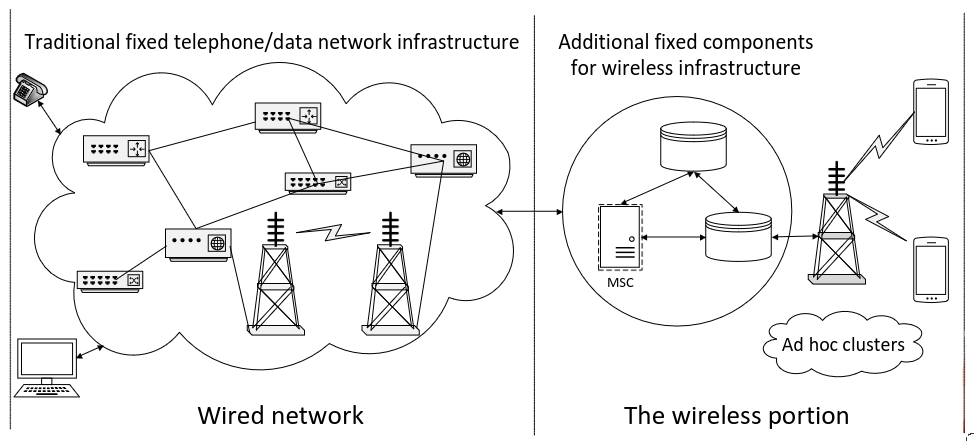
\includegraphics[width=0.5\textwidth]{img/wireless/modern network.png}}
  \end{figure}
  \begin{subsection}{Classification of wireless communication networks}
    Wireless networks can be classified in many ways, but the most common classification is based on
    the coverage area of the network.\\
    They can be also classified by topology or by mobility, as shown in figure \ref{fig:network classification}.
    We will now go over the classification by coverage.
    \begin{figure}[h]
      \centering
      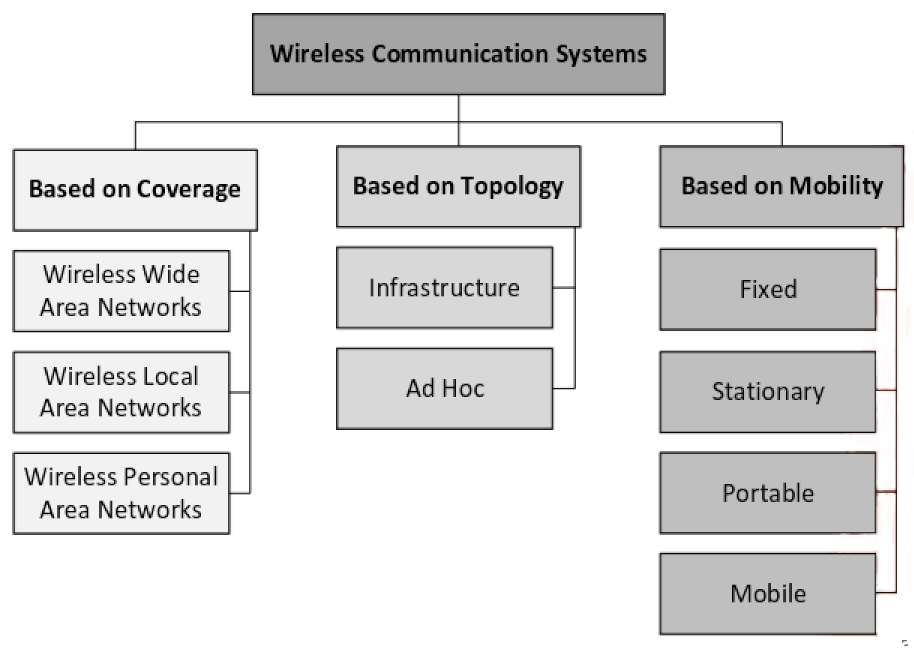
\includegraphics[width=0.7\textwidth]{img/wireless/network classification.png}
      \caption{Classification of wireless networks}
      \label{fig:network classification}
    \end{figure}
    \begin{subsubsection}{Wireless Personal Area Networks}
      A WPAN can be used for communications among the personal devices themselves, adopting an ad-hoc 
      topology.\\
      There are two kinds of ad-hoc networks:
      \begin{itemize}
        \item Master-slave: one device is the master and the others are slaves
        \item Mesh: Nodes are interconnected with wireless links without forming a specific cell
      \end{itemize}
      \begin{figure}
        \centering
        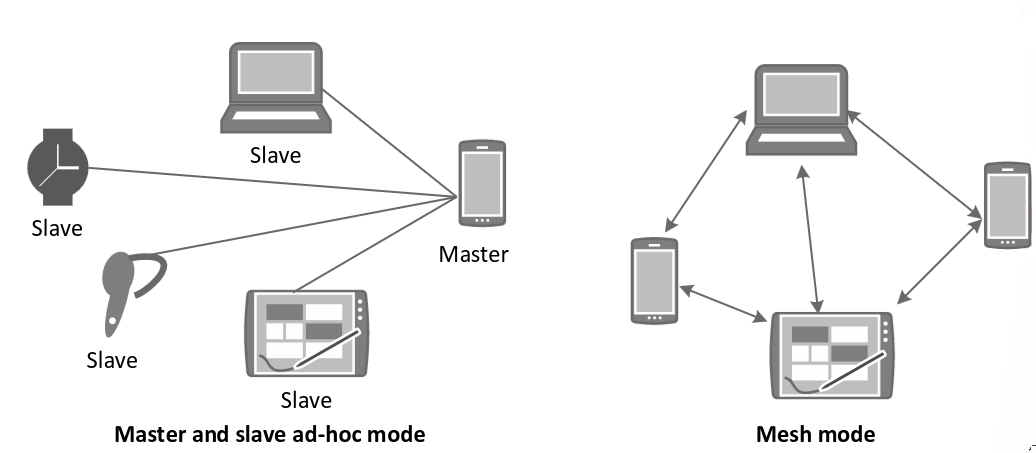
\includegraphics[width=0.7\textwidth]{img/wireless/wpan.png}
        \caption{Wireless Personal Area Network}
      \end{figure}
    \end{subsubsection}
    \begin{subsubsection}{Wireless Local Area Networks}
      A WLAN is a network that covers a small area, such as a home, office, or a campus.\\
      They are normally built on top of a wired local area network (LAN), forming a basic 
      BSS(Basic Service Set), composed of one AP(Access Point) and one or more devices.\\
      A WLAN may have extended service set (ESS) that supports multiple BSSs, similar to a 
      traditional Ethernet based LAN.
    \end{subsubsection}

  \end{subsection}
\end{section}

\begin{section}{Basic security concepts}
  First of all, lets try to define what is \textit{network security}. Well, of course it depends 
  on the context, but in general:
  \begin{boxH}
    \textbf{Network security} is defined as the \textit{protection} of networks and their services from unauthorized
    modification, destruction, or disclosure.
  \end{boxH}
  It provides assurance hat the network performs as expected and in a correct way, with no unexpected 
  side effects.\\
  Network security focuses mainly on networks, network protocols, and network applications, but it 
  also includes all the networks devices and the physical infrastructure.
  \begin{subsection}{Security Threats}
    While traditional networks have no limitations on the coverage, wireless ones have, and its binded
    to the broadcast radio channel.\\
    Wireless networks require decentralized medium access mechanism in medium access
    control (MAC) layer, while also including the means to deal with the mobility of the users.\\
    For those issues, wireless networks make it up with the flexibility and mobility they provide.\\
    Furthermore, the surface of attack is much larger, because the radio waves can be intercepted
    from anywhere in range.\\
    To sum it up, it has many advantages, but also many issues that need to be addressed.
  \end{subsection}
  \begin{subsection}{Security attacks}
    Security is all about dealing with threats and risk, but ideally the system should be designed 
    to address and prevent all possible attacks, but it is not always, or to be honest, almost never possible.\\
    If prevention is not possible, a solution is to detect the attack and then recover from it.\\
    Recall also that an attack is a deliberate action to exploit a vulnerability, which is a 
    \textit{weakness} of a system.\\
    Attacks are formally classified as \textbf{passive attacks} and \textbf{active attacks}:
    \begin{itemize}
      \item Passive attack: the attacker can only read data/traffic
        \subitem \textit{Example}: eavesdropping, can be countered with encryption
        \subitem \textit{Example}: traffic analysis
      \item Active attacker: the attacker can also modify, delete, or create data/traffic
        \subitem \textit{Example}: masquerade, an attacker pretends to be some other entity, usually 
        an authorized user. Can be countered with authentication.
        \subitem \textit{Example}: replay, an attacker first captures a message, (encrypted or not),
        then replays this message to its designated receiver, can be countered with serialization.
        \subitem \textit{Example}: modification of messages, can be countered with integrity of the 
        data, peer authentication, encryption, and serialization(?).
        \subitem \textit{Example}: denial of service
    \end{itemize}
    \begin{figure}[h]
      \centering
      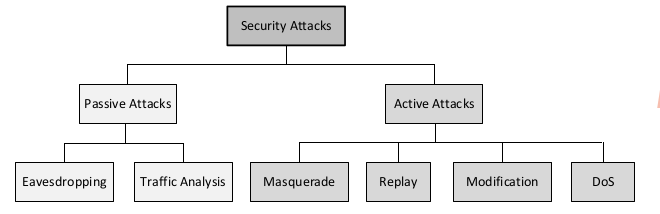
\includegraphics[width=0.7\textwidth]{img/wireless/attacks classification.png}
      \caption{General classification if attacks}
    \end{figure}

    Passive attacks are much harder to detect, because there is no data alteration or system
    manipulation.

  \end{subsection}
  \begin{subsection}{Security Services and proprieties}
    \begin{boxH}
      \textbf{Security services} are the features in a system designed against possible attacks.
    \end{boxH}
    The National Institute of Standards and Technology (NIST) computer security handbook introduces 
    three key security services: confidentiality, integrity, and availability.\\
    We will go over them and some more in the following paragraphs.
    \begin{paragraph}{Access Control}
      Access control is the process of determining what permissions a user should have, and what 
      resources they can access.\\
      this is because the serve should only be accessed by authorized users, and the data should only
      be accessed by authorized users.
    \end{paragraph}
    \begin{paragraph}{Authentication}
      Authentication is the process of verifying the identity of a user.\\
      The goal is to ensure that the user is who they claim to be.
    \end{paragraph}
    \begin{paragraph}{Confidentiality}
      Confidentiality is the process of ensuring that data is only accessible to those who are authorized
      to access it.\\
      This is usually done by encrypting the data.
    \end{paragraph}
    \begin{paragraph}{Integrity}
      Integrity is the process of ensuring that data is not altered in transit.\\
      This is usually done by using checksums or digital signatures.
    \end{paragraph}
    \begin{paragraph}{Non-repudiation}
      Non-repudiation is the process of ensuring that a user cannot deny that they performed a 
      particular action.\\
      This is usually done by using digital signatures.
    \end{paragraph}
    \begin{paragraph}{Availability}
      Availability is the process of ensuring that a system is available when it is needed.\\
      This is usually done by using redundancy and failover systems.
    \end{paragraph}

  \end{subsection}
  \begin{subsection}{Security Mechanisms}
    \begin{boxH}
      Security mechanisms are methods to achieve security services in a system.\\
      They can be implemented in hardware, software, or a combination of both.
    \end{boxH}
    x.800 defines a set of security mechanisms that can be used to achieve the security services
    we talked about before:
    \begin{itemize}
      \item Encryption
      \item Authentication
      \item Access Control
      \item Digital Signatures
    \item Data integrity
    \item Traffic Padding and Routing Control
    \item Notarization
  \end{itemize}
  \begin{paragraph}{Encryption}
    Encryption is the process of encoding data so that only authorized users can read it.\\
    It can provide confidentiality for either data or traffic flow information and can play a part 
    in or complement several other security mechanisms
  \end{paragraph}
  \begin{paragraph}{Authentication}
    In this context, authentication is applied to the message or a party of the communication.
  \end{paragraph}
  \begin{paragraph}{Access Control}
    It is applied to determine and enforce the access rights of the entity depending on the 
    authenticated identity of an entity or information about the entity (such as membership in a 
    known set of entities) or capabilities of the entity.
  \end{paragraph}
  \begin{paragraph}{Digital Signatures}
    This mechanism is used to provide integrity and non-repudiation.
  \end{paragraph}
  \begin{paragraph}{Traffic Padding and Routing Control}
    It can be used to provide various levels of protection against traffic analysis.
  \end{paragraph}
  \begin{paragraph}{Notarization}
    It can be used to provide non-repudiation, and also certificate the destination.
  \end{paragraph}
\end{subsection}
\begin{subsection}{Levels of impact}
  The impact of a security breach can be classified into three levels:
  \begin{itemize}
    \item Low impact: the breach has little or no effect on the assets, operations or individuals.
    \item Moderate impact: the breach has a noticeable effect on the system or the data.
    \item High impact: the breach has severe or catastrophic effects on the system or the data.
  \end{itemize}
\end{subsection}
\begin{boxH}
  IMPORNTANT: After this section there was one of cryptography, but i refuse to explein them over and 
  over again.\\
  Anyway, here's what was explain in case you want to know(\textbf{not} in detail):
  \begin{itemize}
    \item Symmetric encryption
    \item Kerchoff's principle
    \item Adversary model(cipher text only, known plain text, chosen plain text, chosen cipher text)
    \item Asymmetric-key encryption
    \item Classical Ciphers(Ceasar's,Playfair,Vigenère)
    \item monoalphabetic and polyalphabetic ciphers
    \item Stream Cipher(RC4)
    \item Block Cipher(Feistel, DES, 2DES, 3DES)
    \item Steganography
  \end{itemize}
\end{boxH}
\end{section}

\begin{section}{Questions and answers}
  \begin{subsubsection}{Describe the difference between traditional wired and wireless networks.
      List possible classifications for wireless communication systems, providing examples for each
    category.}
    The main difference between the two kinds of network is the link type, in the first one is a
    wired one for all the devices, whereas in the second one it is wired only in the core of the
    network, and wireless for the other nodes.\\
    Wireless networks can be classified by: 
    \begin{itemize}
      \item coverage 
        \begin{itemize}
          \item wide area network
          \item local area network 
          \item personal area network
        \end{itemize}
      \item topology 
        \begin{itemize}
          \item ad-hoc 
          \item infrastructure
        \end{itemize}
      \item mobility
    \end{itemize}
  \end{subsubsection}

  \begin{subsubsection}{Describe the possible security attacks, distinguishing between i) passive
      and ii) active attacks. Which of these are easier to carry out in a wireless network than in a
    wired network? Why?}
    \label{ssec:prev1}
    Some possible security attacks are: 
    \begin{itemize}
      \item eavesdropping(passive): the attacker listen to the messages exchanged between two nodes
      \item traffic analysis(passive):
      \item man-in-the-middle(active): the attacker interposes itself between the two ends of a
        communication and is able to read and manipulate the traffic
      \item spoofing(active): the attacker pretends to be some other entity
      \item denial-of-service(active): refers to the distruption of a service
      \item replay(active): an attaker replays a captured message
    \end{itemize}
    Passive ones are the most simple to carry out, because they do not involve any traffic
    alteration, but only to listen to the logical channel.
  \end{subsubsection}

  \begin{subsubsection}{Consider the confidentiality security service. Define it, and list which
    security mechanisms can be used to provide confidentiality}
    Confidentiality is a security property that refers to the ability to disclose confidential
    information only to authorized users. It is usually carried out by encrypting the exchanged
    data.
  \end{subsubsection}

  \begin{subsubsection}{What are the differences between the security services and the security
    mechanisms?}
    Security services are the set of features in a system which are designed to protect against
    possible attacks, an exemple of this is confidentiality, whereas a security mechanism is a
    method that is used to achieve a security service in a system, like encryption.
  \end{subsubsection}

  \begin{subsubsection}{Define the masquerade and the replay attack. Provide some examples of such
    attacks in the context of wireless networks}
    A masquerade attack consists in a user faking its identity, for exaple to elude address based
    authentication.
    A replay attack consists in sniffing a message and sending it again to the receiver, an example
    of this is a disassociation attack in 802.11.
  \end{subsubsection}

  \begin{subsubsection}{Define the non-repudiation service and a possible mechanism to support it.}
    Non-repudiation is a security property that provides undeniable evidence, usable in a law court,
    of the creator of some data.
    It is usually achieved by implementing a digital signature mechanism.
  \end{subsubsection}

  \begin{subsubsection}{Define the encipherment security mechanism. Provide a list of security
    services it supports.}
  \end{subsubsection}
  \begin{subsubsection}{Define the data integrity security mechanism. Provide a list of security
    services it supports.}
  \end{subsubsection}
  \begin{subsubsection}{Define the traffic padding and routing control security mechanism. Provide a
    list of security services it supports.}
  \end{subsubsection}
  \begin{subsubsection}{What are the main differences between symmetric encryption and asymmetric
    encryption?}
  \end{subsubsection}
  \begin{subsubsection}{Given an alphabet of N symbols, how many possible keys would a simple Caesar
      cypher and a monoalphabetic cypher have? Which attack can an attacker mount to break these two
    cyphers?}
  \end{subsubsection}
  \begin{subsubsection}{Define the polyalphabetic cypher. Given an alphabet of N symbols, how many
    keys will it be possible to generate?}
  \end{subsubsection}
  \begin{subsubsection}{Put in order of security the following cyphers: Polyalphabetic cypher,
    monoalphabetic cypher, Caesar cypher, one-time pad cypher. }
  \end{subsubsection}
  \begin{subsubsection}{Define the completeness, avalanche effect and statistical independence
    properties of the block cypher design criteria}
  \end{subsubsection}
  \begin{subsubsection}{The key of the DES cypher is 56-bits long. What is the length of a
    double-DES and triple-DES algorithms which use k1,k2,k3? Justify your answer.}
  \end{subsubsection}
  \begin{subsubsection}{What are the principles of the asymmetric-key encryption algorithms?}
  \end{subsubsection}
  \begin{subsubsection}{Provide at least two examples of hard problems that can be used to implement
    an asymmetric cypher}
  \end{subsubsection}
  \begin{subsubsection}{Given a plaintext message M and its cyphertext C=Ek(M) obtained with a
      public key encryption. How could an attacker obtain M knowing only C and the public key K? How
    can salting prevent such an attack?}
  \end{subsubsection}
\end{section}
